Плюс критерия Манна-Уитни в том, что он непараметрический, то есть нам не нужно ничего преподалагать о распределнии данных. Еще он менее искажается из-за сильных выборосов, в отличие от критерия Стьюдента.\\ 

\noindent 1. Сначала объединяем значения обоих групп в один массив, сортируем его и присваиваем наблюдениям ранги (важно помнить, что если у вас повторяются значения, то ставится дробный ранг типа 5.5) \\ 
2, Смотрим, каким группам принадлежат наблюдения, и считаем сумму рангов для каждой группы \\ 
3. Считаем статистику $U_{1} = n_{1}*n_{2}\frac{n_{1}(n_{1} + 1)}{2} - R_{1}$ и $U_{2} = n_{1}*n_{2}\frac{n_{2}(n_{2} + 1)}{2} - R_{2}$, где $n_{1}$ и $n_{2}$ -- число наблюдений в каждой из групп, а $R_{1}$ и $R_{2}$ -- ранговые суммы. \\
4. Берем минимальное значение между $U_{1}$ и $U_{2}$. \\ 
5. Ну и сравниваем это значение с критическим значением U (эти значения табличные). Если же полученное значение U больше табличного, принимается нулевая гипотеза о том, что статистически значимой разницы между выборками нет. 

\begin{figure}[H]
	\centering
	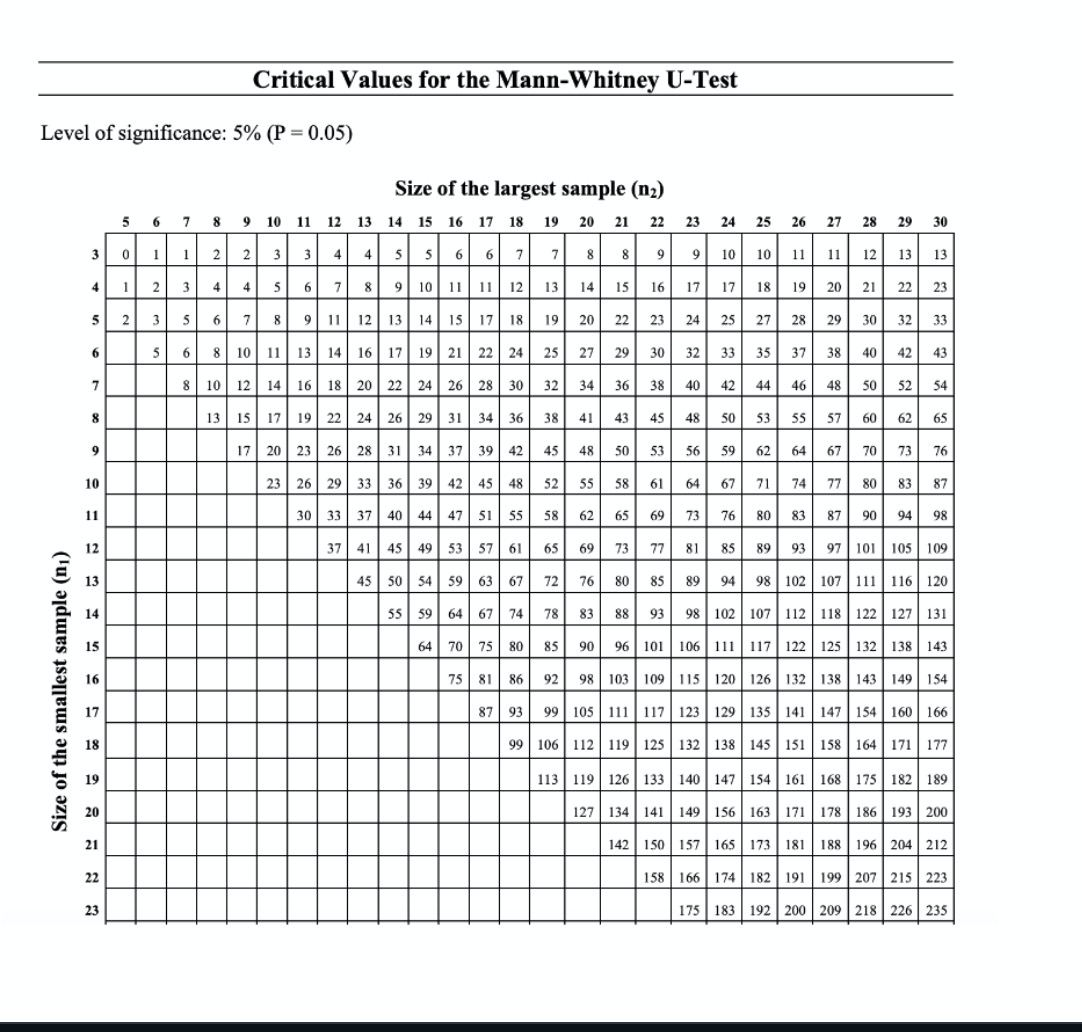
\includegraphics[width=\linewidth]{mannwhitney.jpg}
\end{figure}
	
